\documentclass[11pt,a4paper]{article}
\usepackage[T1]{fontenc}
\usepackage[utf8]{inputenc}
\usepackage[czech]{babel}
\usepackage{lmodern}
\usepackage{geometry}
\geometry{top=27mm,bottom=20mm,left=22mm,right=22mm,headsep=7mm}
\usepackage{amsmath,amssymb,siunitx,graphicx,booktabs,longtable,array,float,caption,microtype,hyperref,xcolor,fancyhdr,enumitem}\hypersetup{hidelinks}
\sisetup{output-decimal-marker={,},exponent-product=\cdot,per-mode=symbol}
\setlength{\parindent}{0pt}
\setlength{\parskip}{4pt}
\captionsetup{font=small,labelfont=bf}
\captionsetup[table]{position=top,skip=6pt}
\captionsetup[figure]{position=bottom,skip=7pt}
\renewcommand{\arraystretch}{1.35}
\setlength{\tabcolsep}{6pt}
\setlength{\arrayrulewidth}{0.45pt}
\pagestyle{fancy}\fancyhf{}
\setlength{\headheight}{25pt}
\newcommand{\labname}{Měření teplotní závislosti rezistivity polovodičového materiálu}
\fancyhead[L]{\footnotesize Pavel Pernička}
\fancyhead[C]{\footnotesize\bfseries Lab 6}
\fancyhead[R]{\parbox[b]{0.49\textwidth}{\raggedleft\footnotesize Měření teplotní závislosti rezistivity polovodiče}}
\fancyfoot[C]{\thepage}
\renewcommand{\headrulewidth}{0.4pt}
\setlist[enumerate]{itemsep=3pt,topsep=3pt}
\begin{document}
\section{Teplotní závislost rezistivity a konduktivity}
Pro zadané teploty jsme změřili napětí a proud vzorkem, ze kterých jsme pro náš vzorek o rezměrech $1{,}5\times4{,}5\times16\,\mathrm{mm}$ vypočítali odpor, rezistivitu a konduktivitu podle následujících vztahů:
$$
R=\frac{U}{I},\qquad \rho=\frac{U}{I}\frac{S}{l},\qquad
\gamma=\frac{1}{\rho},\qquad T=t+273{,}15.
$$

Z rozměrů vzorku jsme získali:
\[
S = a \cdot b
= (1{,}5 \cdot 10^{-3}) \cdot (4{,}5 \cdot 10^{-3})
= 6{,}75 \cdot 10^{-6}\,\mathrm{m^2}.
\]

\[
l = 16\,\mathrm{mm} = 0{,}016\,\mathrm{m}.
\]

Příklad výpočtu pro $t=30\,^{\circ}\mathrm C$:
\[
R=\frac{0{,}1583}{0{,}62753\cdot10^{-3}}
=252{,}26\,\Omega,
\]

\[
\rho=252{,}26\frac{6{,}75\cdot10^{-6}}{0{,}016}
=0{,}10642\,\Omega\,\mathrm m,
\]

\[
\gamma=\frac{1}{0{,}10642}
=9{,}3966\,\mathrm{S/m}.
\]

\begin{table}[H]
\centering
\caption{Naměřené a vypočtené hodnoty pro měřený vzorek}
\small
\setlength{\tabcolsep}{5pt}
\renewcommand{\arraystretch}{1.42}
\begin{tabular}{|r|r|r|r|r|r|}
\hline
$t$ [$^\circ$C] & $U$ [V] & $I$ [mA] & $R$ [$\Omega$] &
$\rho$ [$\Omega\,\mathrm m$] & $\gamma$ [S/m] \\
\hline
30  & 0.1583 & 0.62753 & 252.3 & 0.10642 & 9.3966 \\ \hline
40  & 0.1583 & 0.55566 & 284.9 & 0.12019 & 8.3204 \\ \hline
50  & 0.1583 & 0.51786 & 305.7 & 0.12896 & 7.7544 \\ \hline
60  & 0.1583 & 0.48702 & 325.0 & 0.13713 & 7.2926 \\ \hline
70  & 0.1583 & 0.46613 & 339.6 & 0.14327 & 6.9798 \\ \hline
80  & 0.1583 & 0.44785 & 353.5 & 0.14912 & 6.7061 \\ \hline
90  & 0.1583 & 0.42714 & 370.6 & 0.15635 & 6.3960 \\ \hline
100 & 0.1583 & 0.39034 & 405.5 & 0.17109 & 5.8449 \\ \hline
110 & 0.1583 & 0.37542 & 421.7 & 0.17789 & 5.6215 \\ \hline
120 & 0.1583 & 0.37294 & 424.5 & 0.17907 & 5.5844 \\ \hline
130 & 0.1583 & 0.35058 & 451.5 & 0.19049 & 5.2496 \\ \hline
140 & 0.1583 & 0.33446 & 473.3 & 0.19967 & 5.0082 \\
\hline
\end{tabular}
\end{table}

\begin{figure}[H]\centering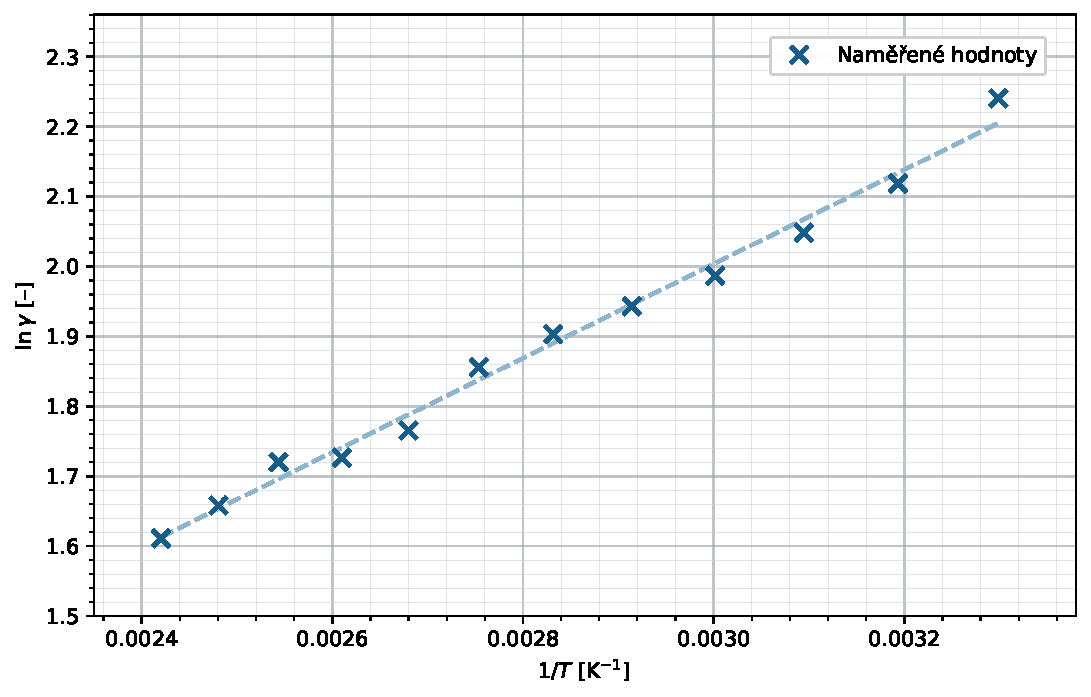
\includegraphics[width=.91\linewidth]{graf1.pdf}\caption{Závislost logaritmu konduktivity na převrácené termodynamické teplotě}\end{figure}

\section{Stanovení koncentrace příměsí}

Koncentraci donorových příměsí ve vzorku určíme
z průměrné konduktivity v teplotním rozsahu 20--80\,°C.
V této oblasti předpokládáme úplnou ionizaci příměsí,
tedy $n \approx N_D$, a zanedbáváme děrovou vodivost.

Pro výpočet použijeme vztah:
\[
\gamma = q N_D \mu_n,
\]
ze kterého vyjádříme koncentraci donorů:
\[
N_D = \frac{\overline{\gamma}}{q\mu_n}.
\]

Kde $N_D$ je koncentrace donorů [m$^{-3}$],
$\overline{\gamma}$ průměrná konduktivita [S/m],
$q = 1{,}602\cdot10^{-19}\,\mathrm C$ je elementární náboj
a $\mu_n = 0{,}135\,\mathrm{m^2\,V^{-1}\,s^{-1}}$
je pohyblivost elektronů v křemíku.

Průměrnou konduktivitu jsme vypočítali jako:
\[
\overline{\gamma}=7{,}7417\,\mathrm{S/m}.
\]

Dosazením získáme koncentraci donorů:
\[
N_D
=\frac{7{,}7417}
{1{,}602\cdot10^{-19}\cdot0{,}135}
=\boxed{3{,}580\cdot10^{20}\,\mathrm{m^{-3}}}.
\]


\newpage
\section{Teplotní závislost vlastní konduktivity křemíku}

Pro teplotní rozsah 150--400\,°C jsme vypočítali konduktivitu
vlastního křemíku podle tohoto vztahu:

\[
\gamma_i(T) =
q N_C (\mu_n+\mu_p)
\exp\left(-\frac{W_g}{2kT}\right).
\]

Kde $\gamma_i$ je konduktivita vlastního polovodiče [S/m],
$q$ je elementární náboj [C], $N_C$ efektivní hustota stavů
ve vodivostním pásu [m$^{-3}$], $\mu_n$ a $\mu_p$ jsou
pohyblivosti elektronů a děr [m$^2$/(V\,s)],
$W_g$ je šířka zakázaného pásu [eV],
$k$ Boltzmannova konstanta [eV/K] a $T$
termodynamická teplota [K].

Pro výpočet byly použity hodnoty:

\[
\begin{aligned}
q &= 1{,}602\cdot10^{-19}\,\mathrm C,\\
N_C &= 2{,}8\cdot10^{25}\,\mathrm{m^{-3}},\\
\mu_n &= 0{,}135\,\mathrm{m^2/(V\,s)},\\
\mu_p &= 0{,}048\,\mathrm{m^2/(V\,s)},\\
W_g &= 1{,}11\,\mathrm{eV},\\
k &= 8{,}6173\cdot10^{-5}\,\mathrm{eV/K}.
\end{aligned}
\]

Příklad výpočtu pro $t=150\,^\circ\mathrm C$:

\[
T=150+273{,}15=423{,}15\,\mathrm K.
\]

\[
\gamma_i = 1{,}602\cdot10^{-19} \cdot2{,}8\cdot10^{25}
\cdot(0{,}135+0{,}048)
\cdot
\exp\left(
-\frac{1{,}11}
{2\cdot8{,}6173\cdot10^{-5}\cdot423{,}15}
\right)\\
\approx 0{,}2007\,\mathrm{S/m}.
\]

Pro celý rozsah jsou výsledkem hodnoty z tabulky \ref{tab:gamma_i}.


\begin{table}[H]
\centering
\caption{Vypočtená teplotní závislost vlastní konduktivity křemíku.}
\label{tab:gamma_i}
\small
\setlength{\tabcolsep}{9pt}
\renewcommand{\arraystretch}{1.4}
\begin{tabular}{|r|r|r|r|r|}
\hline
$t$ [$^\circ$C] & $T$ [K] &
$\gamma_i$ [S/m] &
$1/T$ [K$^{-1}$] & $\ln\gamma_i$ [--] \\
\hline
150 & 423.15 & 0.20143 & 0.00236323 & -1.60233 \\ \hline
175 & 448.15 & 0.47083 & 0.00223140 & -0.75326 \\ \hline
200 & 473.15 & 1.00610 & 0.00211349 & 0.00608 \\ \hline
225 & 498.15 & 1.99215 & 0.00200743 & 0.68921 \\ \hline
250 & 523.15 & 3.69526 & 0.00191150 & 1.30705 \\ \hline
275 & 548.15 & 6.47879 & 0.00182432 & 1.86853 \\ \hline
300 & 573.15 & 10.81608 & 0.00174474 & 2.38103 \\ \hline
325 & 598.15 & 17.29977 & 0.00167182 & 2.85069 \\ \hline
350 & 623.15 & 26.64680 & 0.00160475 & 3.28267 \\ \hline
375 & 648.15 & 39.69879 & 0.00154285 & 3.68132 \\ \hline
400 & 673.15 & 57.41821 & 0.00148555 & 4.05036 \\
\hline
\end{tabular}
\end{table}

Tyto hodnoty byly společně s naměřenou konduktivitou vyneseny do grafu \ref{fig:log}, kde navíc byly proloženy přímkou, která je dále využita pro nalezení průsečíku pro nalezení přechodové teploty (viz níže).

\begin{figure}[H]\centering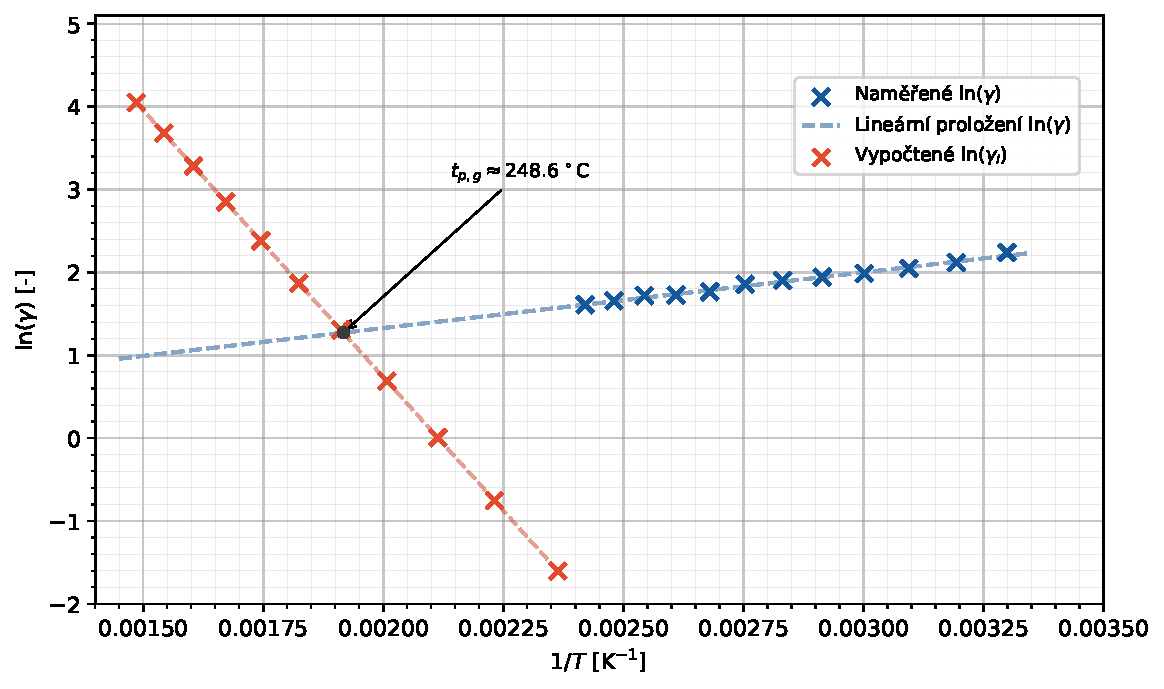
\includegraphics[width=.94\linewidth]{ln_gamma.pdf}\caption{Naměřená závislost logaritmu příměsové a vypočtené vlastní konduktivity na $1/T$, průsečík přechodové teploty.}\label{fig:log}\end{figure}


\section{Určení přechodové teploty}

\subsection{Grafická metoda}

Přechodovou teplotu jsme určili z průsečíku lineárního
proložení naměřené závislosti $\ln\gamma=f(1/T)$
a vypočtené závislosti vlastní konduktivity
$\ln\gamma_i=f(1/T)$.

Z grafu byla určena přibližná přechodová teplota:

\[
t_{p,g} \approx 248{,}6\,^\circ\mathrm C.
\]

Při této teplotě začíná být příspěvek vlastní vodivosti
výrazný ve srovnání s příměsovou vodivostí.

\subsection{Početní metoda}

Početně jsme přechodovou teplotu stanovili ze vztahu:

\[
\overline{\gamma}
= q N_C(\mu_n+\mu_p)
\exp\left(-\frac{W_g}{2kT_p}\right).
\]

Vyjádřením termodynamické teploty ze vztahu získáme:

\[
T_p =
\frac{W_g}
{2k\ln\left(
\frac{qN_C(\mu_n+\mu_p)}
{\overline{\gamma}}
\right)}.
\]

Dosazením:

\[
T_p =
\frac{1{,}11}
{2\cdot8{,}6173\cdot10^{-5}
\cdot\ln\left(
\frac{
1{,}602\cdot10^{-19}\cdot
2{,}8\cdot10^{25}\cdot
(0{,}135+0{,}048)
}{7{,}7417}
\right)}
\]

\[
T_p \approx 556{,}58\,\mathrm K.
\]

Což přepočítáme na stupně Celsia:

\[
t_{p,v} = 556{,}58-273{,}15
=\boxed{283{,}43\,^\circ\mathrm C}.
\]


\section{Zhodnocení}
Při měření teplotní závislosti rezistivity křemíkového polovodiče typu N bylo zjištěno, že v rozsahu 30--140\,°C rezistivita s rostoucí teplotou roste. Tento průběh odpovídá oblasti příměsové vodivosti.
Z~průměrné konduktivity $\overline{\gamma}=7{,}7417\,\mathrm{S/m}$ byla stanovena koncentrace donorů $N_D=3{,}580\cdot10^{20}\,\mathrm{m^{-3}}$. 
Pro vlastní křemík byl vypočten opačný průběh konduktivity, která s rostoucí teplotou výrazně roste díky tepelné generaci párů elektron--díra.

Přechodová teplota byla graficky určena na $248{,}6\,^\circ\mathrm C$ a početní metodou na $283{,}4\,^\circ\mathrm C$. Rozdíl přibližně $35\,^\circ\mathrm C$ je způsoben odlišným způsobem aproximace příměsové vodivosti. Přesnost výsledků mohla ovlivnit také nepřesnost měření proudu, napětí a hlavně teploty vzorku kvůli nutnosti manuálního odečtu z kapalinového sloupce. 
Navíc, jelikož přechodová teplota leží mimo měřený rozsah, je pouze odhadem.

\end{document}
